\documentclass[a4paper, oneside]{scrreprt}
\usepackage[utf8]{inputenc}
\usepackage{graphicx}
\inputencoding{utf8}
\author{Andre Brand}
\author{Marcel Lange}

\begin{document}
    \title{Dokumentation zur Aufgabe 2}
	\author{Andre Brand, Marcel Lange}
    \date{Version 1.1}
    \subject{Praktikum Rechnernetze}
    \maketitle

	\renewcommand{\contentsname}{Inhaltsverzeichnis}
    \tableofcontents

\chapter{Einführung}
Im Rahmen der Verantaltung "Rechnernetze" im Wintersemester 2017/2018 an der HAW Hamburg soll ein Chatprogramm mit einem eigenen Protokoll implementiert werden.
Im folgenden werden wir über das Protokoll, sowie über die Implementierung der Server-Anwendung und die Client-Anwendung schreiben. 

\section{Allgemeines}
Wir entschieden uns dafür, ein Chatprogramm zu erstellen, dass die Benutzernamen nicht speichert. Man kann sich also nicht einen festen Benutzernamen sichern und man muss sich nicht registrieren.
\\Neue Chaträume können nur durch die Server-Andwendung erstellt werden. Benutzer können mit Hilfe eines Befehlswortes einen Chat-Raum und mit einem anderen ihren Namen wechseln.  
\\Die Nachrichten der Benutzer dürfen alle Zeichen des UTF8-Standarts beinhalten.
\\Der Chat wird über eine TCP-Verbindung realisiert und es werden Zeichenketten übermittelt. Mit bestimmten Befehlen, die sich immer am Anfang der Zeichenkette befinden und mit einem '\$' eingeleitet werden, können zum Beispiel der Benutzername geändert oder der Chatraum gewechselt werden. Wird in dieser Zeichenkette kein Befehl erkannt, wird es als normale Chatnachricht an den Server weitergeleitet.

\section{Client}
Der Client wird dem ''DEFAULT'' Chatraum zugewiesen. Der Chat-Client kann eine Liste aller
sich in seinem Raum befindenden Benutzer anfordern, sowie eine Liste aller Chaträume. Der
Chat-Client kann ebenfalls seinen Chatraum wechseln.
\\Ein Chat-Client kann, sobald er sich in einem Chatraum befindet, Nachrichten an alle anderen
Benutzer in diesem Raum senden, ohne auf eine Antwort des Servers warten zu müssen.
\newpage

\chapter{Befehle}
\begin{itemize}
\item \textbf{\$DISCONNECT} - Anfrage des Benutzers an den Server, der daraufhin denn ''Account'' Thread, alle Streams und den Socket schließt und alle anderen Benutzer im Chatraum benachrichtigt.
\item \textbf{\$USERLIST} - Anfrage des Benutzers an den Server, der daraufhin alle Namen der Benutzer zurücksendet, die sich im selben ChatRaum befindet. Die erste Zeile, die der Server sendet ist "Userlist:" und die letzte Zeile ist "End". Dazwischen werden zeilenweise die Usernames gesendet. 
\item \textbf{\$ROOMLIST} - Anfrage des Benutzers an der Server, der daraufhin die Namen alle verfügbaren Chaträume zurücksendet. Die erste Zeile, die der Server sendet ist ''Available Chatrooms: '' und die letzte Zeile ist "End". Dazwischen werden zeilenweise die Namen der Chaträume gesendet.
\item \textbf{\$ROOMJOIN$<$!$>$[Raumname]} - Anfrage des Benutzers an der Server, der den Benutzer in den Chatraum mit dem angegebenen Namen transferiert sofern dieser existiert. War das Transferieren erfolgreich, wird eine Nachricht im Format ''[Username] Joined [NeuerRaum]'' an alle Benutzer des neuen Chatraumes gesendet. Sollte der übergebene Chatraum nicht existieren wird die Fehlermeldung ''ROOMJOIN FAILED'' an den Benutzer gesendet. Sollte ein Syntaxfehler auftreten antwortet der Server mit ''wrong syntax: \$ROOMJOIN$<$!$>$CHATROOM''.
\item \textbf{\$SETNAME$<$!$>$[Username]} - Ändert denn Username in ''Username''. Der Username kann
sowohl groß als auch klein geschrieben werden (muss eindeutig sein). War der Wechsel des Benutzernamen erfolgreich, wird eine Nachricht vom Server im Format ''[AlterBenutzerName] changed Name to [NeuerBenutzerName]'' an alle Nutzer im Chatraum gesendet. Ist der Benutzername auf dem Server schon vorhanden, sendet der Server als Antwort ''SETNAME FAILED''. Sollte ein Syntaxfehler auftreten antwortet der Server mit ''wrong syntax: \$SETNAME$<$!$>$USERNAME''.
\item \textbf{\$COMMANDLIST} - Anfrage an den Server, der daraufhin alle Befehle zurück sendet. Die erste Zeile, die der Server sendet ist "Commandlist:" und die letzte Zeile ist ''End''. Dazwischen werden zeilenweise die Befehle gesendet.
\item \textbf{\$CURRENTROOM} - Anfrage an den Server, der daraufhin den Namen des Chatraumes zurücksendet, in dem der Benutzer sich befindet. 
\item Normale Chat-Nachrichten werden ohne Befehl gesendet und vom Server an alle Benutzer innerhalb des Chatraumes gesendet.
\end{itemize}
Sollte ein Befehl nicht erkannt werden, da er z.B. falsch geschrieben wurde, wird er als Chat-Nachricht interpretiert und an alle Benutzer des Chatraumes gesendet.
\newpage

\chapter{Architektur des Servers}
Wenn der Server gestartet wird, wird direkt ein Server-Socket erstellt, der auf eingehende Verbindungen wartet. \\
Wenn eine Verbindung hergestellt wird, erstellt der ServerSocket einen Client, der Serverseitig läuft. Für diesen Client wird ein Thread gestartet, in dem die Nachrichten empfangen, ausgewertet und versendet werden. \\
Jeder Thread repräsentiert hierbei einen Benutzer. Wenn sich der Benutzer an einem ChatRaum anmeldet, dann wird der Thread als Observer dem ChatRaum zugewiesen, welcher das Interface Observable implementiert. Neue Nachrichten werden dann über die Methode \textbf{notifyObservers()} an die serverseitigen Clients weitergeleitet, welche die Nachricht über das Protokoll an die Clients der Benutzer weiterleiten.\\

\section{UML Diagram des Servers}

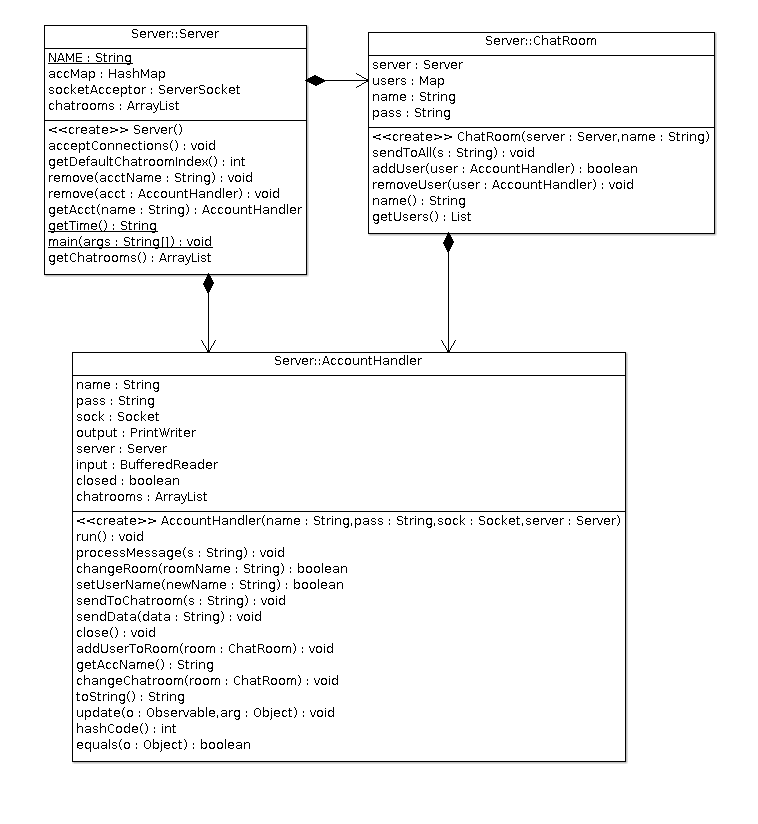
\includegraphics[scale=0.6]{data/RNPA2Server.png}


\chapter{Architektur der Clients}
Die Clients des Benutzer-Programms beinhalten einen Listener, der als Thread am Socket nach neuen Nachrichten horcht. Neue Nachrichten werden vom Listener über das Observer-Pattern an den Client weitergeleitet. Die GUI wird dann auf dem gleichen Weg vom Client benachrichtig.\\
Neue Nachrichten werden lediglich über die Klasse ChatClient versendet.

\section{UML-Diagram des Clients}

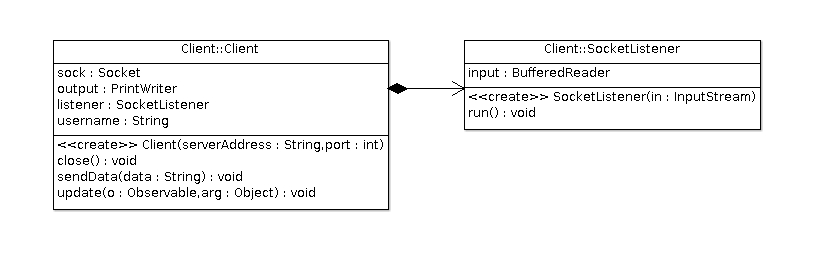
\includegraphics[scale=0.6]{data/RNPA2Client.png}

\end{document}